\chapter{时间演化、守恒与耦合自旋}

量子态并非希尔伯特空间中的一个固定点。随着时间推移它会移动，但它的移动不能丢失归一化、概率或内积所编码的可区分性。这些要求几乎决定了量子动力学的形式。线性给出一个时间演化算符，概率守恒使该算符成为幺正的，而无穷小幺正变换由一个厄米算符生成。这个算符就是哈密顿量。我们将从这些陈述出发推导Schr\"odinger方程，考察能量本征态如何积累相位，然后把这一形式体系转化为两个具体计算：一个自旋在磁场中的进动，以及一对耦合自旋的两个态之间的振荡。

\section{希尔伯特空间中的线性运动}

设时刻\(t\)的态为\(\ket{\psi(t)}\)。我们假设它与零时刻态的关系是线性的：
\begin{equation}
\ket{\psi(t)}=U(t)\ket{\psi(0)}.
\end{equation}
线性是一条公设，而不是从更基本的东西推导出来的定理。它是量子力学中经实验证实的一部分，而试图取代它通常会危及概率或守恒定律。在选定的基下，\(U(t)\)不过是一个依赖于时间的矩阵。

对偶矢量遵循共轭规则。若
\begin{equation}
\ket{\phi(t)}=U(t)\ket{\phi(0)},
\end{equation}
则
\begin{equation}
\bra{\phi(t)}=\bra{\phi(0)}U^\dagger(t).
\end{equation}
对于矩阵，匕首号表示先复共轭再转置。因此，左矢在对偶空间中承载着与右矢相同的演化规律。

\subsection{概率守恒意味着幺正性}

归一化的态表示总概率为一：
\begin{equation}
\braket{\psi(t)}{\psi(t)}=1.
\end{equation}
时间演化必须保持这个范数。事实上，一个保持每个矢量范数的线性映射也保持每个内积。从几何上看，保持两个矢量及其差矢量的长度，就保持了它们构成的三角形，从而保持它们的夹角。在复矢量空间中，只要再考虑带有因子\(i\)的组合，就能得到同样的结论。

因此，对于任意的\(\ket{\phi}\)和\(\ket{\psi}\)，
\begin{equation}
\braket{\phi(t)}{\psi(t)}
=
\braket{\phi(0)}{\psi(0)}.
\end{equation}
代入演化规律得到
\begin{equation}
\bra{\phi(0)}U^\dagger(t)U(t)\ket{\psi(0)}
=
\braket{\phi(0)}{\psi(0)}.
\end{equation}
由于这个方程对每一对矢量都成立，
\begin{equation}
\boxed{U^\dagger(t)U(t)=I}.
\end{equation}
这样的算符是幺正的。其标量类比是模为1的复数，
\begin{equation}
e^{i\theta}\bigl(e^{i\theta}\bigr)^*=1.
\end{equation}
幺正算符是纯相位的矩阵推广：它可以让一个态在希尔伯特空间中旋转，但不能拉伸或压缩它。

\section{无穷小生成元}

有限演化由非常小的时间步长构建而成。设经过的时间为\(\epsilon\)，小到可以忽略\(\epsilon^2\)阶的项。在零经过时间时什么也没有发生，所以
\begin{equation}
U(0)=I.
\end{equation}
领头修正项必须正比于\(\epsilon\)。我们按惯例把它写成
\begin{equation}
\boxed{U(\epsilon)=I-\frac{i\epsilon}{\hbar}H}.
\end{equation}
在这一阶段，只有\(\epsilon\)这个因子是被迫的。\(i\)、\(\hbar\)以及\(H\)这个名称的选取，是为了让最后留下的对象具有标准归一化并且是厄米的。

\begin{classroomqa}
\lecturetimestamp{00:12:46}
\audiencequestion{为什么普朗克常数在熟悉的单位中是一个如此小得惊人的数？}
\lecturerresponse{其数值大小反映了人类所选择的单位。化学家选取的是能装进手边容器中的宏观量，而原子比人小得多。在适应这些宏观尺度的单位中，一个原子的作用量子必然显得极小。这并不是一个独立的动力学之谜；它在很大程度上是单位中所固有的人类历史尺度。}
\end{classroomqa}

取厄米共轭，
\begin{equation}
U^\dagger(\epsilon)
=I+\frac{i\epsilon}{\hbar}H^\dagger.
\end{equation}
现在相乘并只保留一阶项：
\begin{align}
U^\dagger(\epsilon)U(\epsilon)
&=
\left(I+\frac{i\epsilon}{\hbar}H^\dagger\right)
\left(I-\frac{i\epsilon}{\hbar}H\right) \\
&=
I+\frac{i\epsilon}{\hbar}\left(H^\dagger-H\right)
+O(\epsilon^2).
\end{align}
幺正性要求这个乘积等于\(I\)，因此
\begin{equation}
\boxed{H^\dagger=H}.
\end{equation}
时间演化的无穷小生成元是厄米的。由于厄米算符表示可观测量，每个动力学系统都拥有一个生成其时间运动的可观测量。这就是哈密顿量。我们用\(H\)表示该算符，而把\(E\)留给它可能的测量值，即本征值。

\begin{classroomqa}
\lecturetimestamp{00:18:34}
\audiencequestion{为什么这个生成元应该被称为能量？能量难道不是\(p^2/2m\)，或者说做功的能力吗？}
\lecturerresponse{那些是在特殊的经典情形中有用的描述，而不是一般定义。表达式\(p^2/2m\)只是非相对论自由粒子的动能，它并不能定义诸如储存在电磁场中的能量之类的东西。对于一个抽象系统，对能量所要求的第一个普遍特征就是守恒。我们很快将证明\(H\)的期望值是守恒的，而其本征态的相位也将满足\(E=\hbar\omega\)。这两个事实把该生成元与能量等同起来。}
\end{classroomqa}

\section{从一小步到Schr\"odinger方程}

无穷小更新其实已经是一个伪装起来的微分方程。在任意的时间原点处，
\begin{equation}
\frac{d}{dt}\ket{\psi(t)}
=
\lim_{\epsilon\to0}
\frac{\ket{\psi(t+\epsilon)}-\ket{\psi(t)}}{\epsilon}.
\end{equation}
板书上首先在\(t=0\)处写出它；移动原点便得到上面的普遍形式。

\begin{figure}[htbp]
\centering
\includegraphics[width=0.72\textwidth]{lecture_09_figure_03.png}
\caption{将无穷小演化转化为微分方程的差商。}
\lectureframe{00:22:15}
\end{figure}

利用
\begin{equation}
\ket{\psi(t+\epsilon)}
=
\left(I-\frac{i\epsilon}{\hbar}H\right)\ket{\psi(t)}.
\end{equation}
于是
\begin{align}
\frac{d}{dt}\ket{\psi(t)}
&=
\lim_{\epsilon\to0}
\frac{\left(I-\frac{i\epsilon}{\hbar}H\right)\ket{\psi(t)}
-\ket{\psi(t)}}{\epsilon} \\
&=
-\frac{i}{\hbar}H\ket{\psi(t)}.
\end{align}
等价地，
\begin{equation}
\boxed{
i\hbar\frac{d}{dt}\ket{\psi(t)}
=H\ket{\psi(t)}
}.
\end{equation}
这就是Schr\"odinger方程。一旦\(H\)以及某一时刻的态已知，它就确定了此后各时刻的态。随后测量的概率则由通常的测量规则给出。

\section{能量本征态与旋转相位}

最简单的解从哈密顿量的一个本征矢量开始：
\begin{equation}
H\ket{\psi_E}=E\ket{\psi_E}.
\end{equation}

\begin{figure}[htbp]
\centering
\includegraphics[width=0.70\textwidth]{lecture_09_figure_04.png}
\caption{黑板上的能量本征值方程。}
\lectureframe{00:28:22}
\end{figure}

由于\(H\)把\(\ket{\psi_E}\)送回同一个一维方向，时间演化不能把它与另一个本征矢量混合。它只能乘以一个标量：
\begin{equation}
\ket{\psi_E(t)}=f(t)\ket{\psi_E}.
\end{equation}
代入Schr\"odinger方程给出
\begin{align}
i\hbar\,\dot f(t)\ket{\psi_E}
&=
f(t)H\ket{\psi_E} \\
&=
E f(t)\ket{\psi_E}.
\end{align}
因此
\begin{equation}
\dot f(t)=-\frac{iE}{\hbar}f(t),
\qquad
f(t)=e^{-iEt/\hbar},
\end{equation}
以及
\begin{equation}
\boxed{
\ket{\psi_E(t)}
=e^{-iEt/\hbar}\ket{\psi_E(0)}
}.
\end{equation}
能量本征态是定态的，意思是它在希尔伯特空间中的射线不移动。然而它的右矢会累积相位。

指数可以写成
\begin{equation}
e^{-iEt/\hbar}
=
\cos\!\left(\frac{Et}{\hbar}\right)
-i\sin\!\left(\frac{Et}{\hbar}\right).
\end{equation}
负号以及正弦内缺少额外的\(i\)，是在黑板计算过程中修正的。角频率为
\begin{equation}
\omega=\frac{E}{\hbar},
\qquad
\boxed{E=\hbar\omega}.
\end{equation}
等价地，用普通频率\(\nu=\omega/(2\pi)\)，有\(E=h\nu\)。

\begin{figure}[htbp]
\centering
\includegraphics[width=0.78\textwidth]{lecture_09_figure_05.png}
\caption{相位解与能量--频率关系在相邻的黑板上展开。}
\lectureframe{00:36:19}
\end{figure}

\begin{classroomqa}
\lecturetimestamp{00:34:43}
\audiencequestion{为什么在计算需要之前就把因子\(i\)和\(\hbar\)插入无穷小算符中？}
\lecturerresponse{它们是以答案为出发点选定的约定。没有\(i\)，幺正性会使生成元成为反厄米的。乘以\(i\)把它变成具有实本征值的厄米可观测量。因子\(\hbar\)赋予这些本征值能量的单位和归一化约定。物理陈述是幺正性；这些因子把它的生成元化为标准形式。}
\end{classroomqa}

\begin{classroomqa}
\lecturetimestamp{00:36:18}
\audiencequestion{\(E=\hbar\omega\)只属于电磁波和光子吗？}
\lecturerresponse{不。光子是一个重要的情形，但该关系更为普遍。任何哈密顿量本征态都会获得角频率为\(E/\hbar\)的相位。把电磁场模式的频率与其光子的频率联系起来需要更多物理，但能量--相位关系本身已经由量子时间演化得出。}
\end{classroomqa}

\section{能量基中的叠加}

单个能量本征态只发生整体相位变化，而整体相位不能影响概率。当态包含若干能量本征矢量时，有趣的动力学才开始。由于厄米哈密顿量具有完备正交归一本征基，
\begin{equation}
H\ket{\psi_n}=E_n\ket{\psi_n},
\qquad
\ket{\psi(0)}=\sum_n\alpha_n\ket{\psi_n}.
\end{equation}

\begin{figure}[htbp]
\centering
\includegraphics[width=0.72\textwidth]{lecture_09_figure_06.png}
\caption{任意态在哈密顿量本征矢量中的展开。}
\lectureframe{00:38:35}
\end{figure}

线性性允许每个分量各自演化：
\begin{equation}
\boxed{
\ket{\psi(t)}
=
\sum_n\alpha_n e^{-iE_n t/\hbar}\ket{\psi_n}
}.
\end{equation}
高能分量在复平面上快速旋转；低能分量旋转得更慢。改变可测概率的，不是整个态共享的相位，而是具有不同\(E_n\)的分量之间不断变化的相对相位。

在能量基中，
\begin{equation}
\begin{aligned}
H&=
\begin{pmatrix}
E_1&0&\cdots\\
0&E_2&\cdots\\
\vdots&\vdots&\ddots
\end{pmatrix},\\[0.6em]
U(t)&=
\begin{pmatrix}
e^{-iE_1t/\hbar}&0&\cdots\\
0&e^{-iE_2t/\hbar}&\cdots\\
\vdots&\vdots&\ddots
\end{pmatrix}.
\end{aligned}
\end{equation}
对于不依赖时间的哈密顿量，同一陈述可以不选择基而概括为
\begin{equation}
\boxed{U(t)=e^{-iHt/\hbar}},
\end{equation}

\begin{classroomqa}
\lecturetimestamp{00:40:17}
\audiencequestion{这种分解本质上是一个傅里叶级数吗？它是否类似于热传导中使用的分解？}
\lecturerresponse{它确实是一种时间上的类傅里叶分解：每个能量本征矢量带有确定的频率。傅里叶方法和拉普拉斯方法也在许多经典方程中分离模式，包括扩散。数学上的相似是真实的，但关于哪个物理量对应于频率的主张必须逐例检验。在量子力学中，具体关系由Schr\"odinger方程固定。}
\end{classroomqa}

\subsection{组合系统}

对于两个非相互作用系统 \(A\) 和 \(B\)，组合哈密顿量是乘积空间上各自生成元的和：
\begin{equation}
H_{AB}
=
H_A\otimes I_B+I_A\otimes H_B.
\end{equation}
如果
\begin{equation}
H_A\ket{a}=E_a\ket{a},
\qquad
H_B\ket{b}=E_b\ket{b},
\end{equation}
那么
\begin{equation}
H_{AB}\ket{a,b}=(E_a+E_b)\ket{a,b}.
\end{equation}
对于分离的非相互作用系统，能量因而相位频率相加。相互作用会贡献另一项 \(H_{\mathrm{int}}\)，因此这个简单的和不再给出全部能量。

\begin{classroomqa}
\lecturetimestamp{00:56:20}
\audiencequestion{如果两个分离的系统包含具有相同频率的分量，当把它们放在一起时会发生什么？}
\lecturerresponse{对于非相互作用系统，组合能量本征值是各自本征值之和。两个频率相等可能产生简并，但它本身并不混合相应的本征向量。混合需要相互作用项或在简并子空间内选择一组基。一旦系统发生相互作用，就必须把扩大后的哈密顿量作为一个新问题来对角化。}
\end{classroomqa}

\section{期望值与对易子}

我们一直保持可观测量固定来跟踪态。这就是 Schr\"odinger 绘景。设 \(A\) 是一个没有显式时间依赖性的可观测量。它的期望值是
\begin{equation}
\langle A\rangle_t
=
\bra{\psi(t)}A\ket{\psi(t)}.
\end{equation}
对左矢和右矢都求导：
\begin{equation}
\frac{d}{dt}\langle A\rangle_t
=
\bra{\dot\psi}A\ket{\psi}
+
\bra{\psi}A\ket{\dot\psi}.
\end{equation}
Schr\"odinger 方程及其厄米共轭给出
\begin{equation}
\ket{\dot\psi}
=-\frac{i}{\hbar}H\ket{\psi},
\qquad
\bra{\dot\psi}
=\frac{i}{\hbar}\bra{\psi}H.
\end{equation}
因此
\begin{align}
\frac{d}{dt}\langle A\rangle_t
&=
\frac{i}{\hbar}\bra{\psi}HA\ket{\psi}
-\frac{i}{\hbar}\bra{\psi}AH\ket{\psi} \\
&=
\frac{i}{\hbar}\bra{\psi}(HA-AH)\ket{\psi}.
\end{align}
定义对易子
\begin{equation}
[H,A]=HA-AH.
\end{equation}
那么期望值的运动方程是
\begin{equation}
\boxed{
\frac{d}{dt}\langle A\rangle_t
=
\frac{i}{\hbar}\langle[H,A]\rangle_t
}.
\end{equation}

\begin{figure}[htbp]
\centering
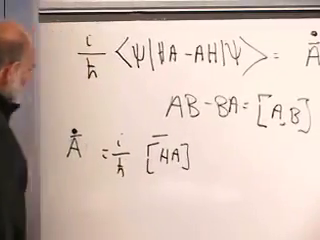
\includegraphics[width=0.74\textwidth]{lecture_09_figure_07.png}
\caption{期望值方程与对易子 \(AB-BA=[A,B]\)。}
\lectureframe{00:51:05}
\end{figure}

\begin{classroomqa}
\lecturetimestamp{00:49:13}
\audiencequestion{为什么这个方程中的对易子本身也在一个期望值里面？}
\lecturerresponse{对易子是一个算符。任何放在 \(\bra{\psi}\) 和 \(\ket{\psi}\) 之间的算符都有一个期望值，所以 \(\bra{\psi}[H,A]\ket{\psi}\) 只是该对易子在当前态中的平均值。}
\end{classroomqa}

\subsection{守恒定律}

令 \(A=H\)。一个算符总是与自身对易：
\begin{equation}
[H,H]=HH-HH=0.
\end{equation}
因此
\begin{equation}
\boxed{
\frac{d}{dt}\langle H\rangle_t=0
}.
\end{equation}
哈密顿量的期望值是守恒的。这就是所承诺的、把 \(H\) 认定为能量的结构性理由。每个孤立系统都有一个哈密顿量，而每个不依赖时间的哈密顿量都提供这条守恒定律。

更一般地，
\begin{equation}
[H,A]=0
\quad\Longrightarrow\quad
\frac{d}{dt}\langle A\rangle_t=0.
\end{equation}

\begin{classroomqa}
\lecturetimestamp{00:51:41}
\audiencequestion{与 \(H\) 对易的所有算符的集合，其物理解释是什么？它是否包含能量之外的量？}
\lecturerresponse{它们是系统的守恒可观测量。哪些会出现取决于哈密顿量。自由粒子守恒动量，而力可以破坏这种守恒。能量总是存在，因为 \(H\) 与自身对易；额外的对易算符表达额外的对称性和守恒定律。}
\end{classroomqa}

\section{磁场中的一个自旋}

考虑一个自旋，其泡利算符为
\begin{equation}
\boldsymbol{\sigma}
=(\sigma_1,\sigma_2,\sigma_3)
\end{equation}
它处于固定的外磁场 \(\mathbf B\) 中。磁矩与自旋成正比。在本文使用的约定中，
\begin{equation}
\boxed{
H=\frac{\mu}{2}\boldsymbol{\sigma}\cdot\mathbf B
}.
\end{equation}
因子 \(1/2\)、符号以及依赖电荷的标度都可以吸收到 \(\mu\) 的定义中。磁场按经典方式处理：一块大而稳定的磁体提供 \(\mathbf B\)，而我们不建模该磁体的量子态。

\begin{figure}[htbp]
\centering
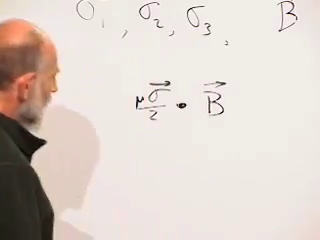
\includegraphics[width=0.68\textwidth]{lecture_09_figure_08.png}
\caption{磁矩算符与外磁场耦合。}
\lectureframe{01:01:45}
\end{figure}

选择磁场沿第三轴，
\begin{equation}
\mathbf B=B\hat{\mathbf z},
\qquad
H=\frac{\mu B}{2}\sigma_3.
\end{equation}
我们将跟踪三个自旋分量的期望值。为缩短方程，记
\begin{equation}
s_i(t)=\langle\sigma_i\rangle_t.
\end{equation}
纵向分量满足
\begin{equation}
\dot s_3
=
\frac{i}{\hbar}\langle[H,\sigma_3]\rangle
=0,
\end{equation}
因为 \(H\) 与 \(\sigma_3\) 成正比。自旋沿磁场的投影是固定的。几何上，平均自旋的尖端必须保持在围绕磁场轴、具有固定张角的圆锥面上。

\begin{figure}[htbp]
\centering
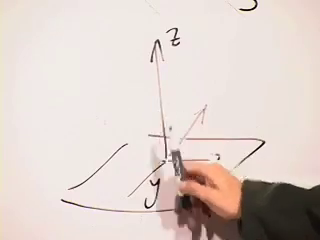
\includegraphics[width=0.58\textwidth]{lecture_09_figure_09.png}
\caption{固定的纵向自旋使运动保持在围绕磁场轴的圆锥面上。}
\lectureframe{01:04:45}
\end{figure}

对于第一个横向分量，
\begin{equation}
\dot s_1
=
\frac{i\mu B}{2\hbar}
\langle[\sigma_3,\sigma_1]\rangle.
\end{equation}
该对易子可以直接由下式检验
\begin{equation}
\begin{aligned}
\sigma_3&=
\begin{pmatrix}1&0\\0&-1\end{pmatrix},
&
\sigma_1&=
\begin{pmatrix}0&1\\1&0\end{pmatrix},\\[0.5em]
\sigma_2&=
\begin{pmatrix}0&-i\\i&0\end{pmatrix}.
\end{aligned}
\end{equation}
确实，
\begin{equation}
\sigma_3\sigma_1=i\sigma_2,
\qquad
\sigma_1\sigma_3=-i\sigma_2,
\end{equation}
所以
\begin{equation}
[\sigma_3,\sigma_1]=2i\sigma_2.
\end{equation}
因此，
\begin{equation}
\dot s_1=-\frac{\mu B}{\hbar}s_2.
\end{equation}
同样，利用 \([\sigma_3,\sigma_2]=-2i\sigma_1\)，
\begin{equation}
\dot s_2=\frac{\mu B}{\hbar}s_1.
\end{equation}

\begin{figure}[htbp]
\centering
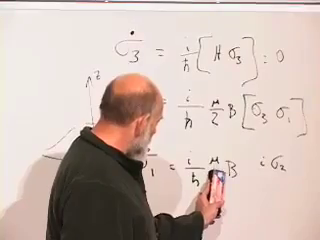
\includegraphics[width=0.72\textwidth]{lecture_09_figure_10.png}
\caption{导致横向运动方程的泡利对易子计算。}
\lectureframe{01:09:35}
\end{figure}

令
\begin{equation}
\Omega=\frac{\mu B}{\hbar}.
\end{equation}
这三个方程是
\begin{equation}
\dot s_1=-\Omega s_2,
\qquad
\dot s_2=\Omega s_1,
\qquad
\dot s_3=0.
\end{equation}
一个横向振幅为 \(s_\perp\) 的解是
\begin{equation}
s_1(t)=s_\perp\cos(\Omega t+\varphi),
\qquad
s_2(t)=s_\perp\sin(\Omega t+\varphi),
\end{equation}
其中 \(s_3\) 为常数。

\begin{figure}[htbp]
\centering
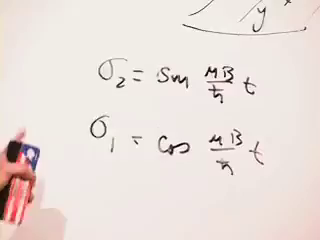
\includegraphics[width=0.64\textwidth]{lecture_09_figure_11.png}
\caption{横向自旋分量构成一对正弦--余弦，其角频率为 \(\mu B/\hbar\)。}
\lectureframe{01:11:45}
\end{figure}

因此，平均自旋像陀螺一样绕磁场进动。选择磁场沿\(z\)方向只是为了方便。对于任意方向的磁场，平行于\(\mathbf B\)的分量守恒，而垂直分量绕其旋转。

\begin{classroomqa}
\lecturetimestamp{01:13:02}
\audiencequestion{正弦和余弦解是否应包含一个额外的相位？}
\lecturerresponse{是的。相位\(\varphi\)指定了横向平面内的初始方向，或者等价地，指定了被称为\(t=0\)的时刻的选择。将其设为零只是选择自旋从某一特定横向轴开始。}
\end{classroomqa}

\subsection{制备与测量}

假设一个系综被制备在\(\sigma_1\)的\(+1\)本征态。在\(t=0\)时，对\(\sigma_1\)的测量必定返回\(+1\)，而对\(\sigma_2\)或\(\sigma_3\)的测量给出\(\pm1\)的等概率。经过四分之一进动周期后，态已旋转到\(\sigma_2\)的\(+1\)本征态：此时\(\sigma_2\)是确定的，而\(\sigma_1\)是完全不确定的。再经过四分之一周期，它到达\(\sigma_1\)的\(-1\)本征态。因此，旋转的期望值具有直接的操作意义。

\begin{classroomqa}
\lecturetimestamp{01:14:04}
\audiencequestion{如果期望值需要许多电子，系综的成员难道不会携带不同的相位并抵消进动吗？}
\lecturerresponse{当对每个成员进行相同的实验时，不会。相同的制备使每个电子具有相同的初始态，因而具有相同的相位演化。如果它们的初始相位不受控制，该系综就不是纯制备；它是混合态，退相位可能减小横向平均值。}
\end{classroomqa}

\section{两个耦合自旋}

现在考虑两个自旋。仅仅说它们纠缠不足以预测它们将如何运动。动力学需要一个哈密顿量。

\begin{classroomqa}
\lecturetimestamp{01:16:49}
\audiencequestion{如果两个电子纠缠，使得沿任意共同轴测量都得到相反的结果，这是否意味着它们的运动总是相位相差\(180^\circ\)？}
\lecturerresponse{仅凭纠缠不能得出任何动力学结论。所述的反关联描述的是单态，但其后续演化取决于能量算符。我们必须首先明确是否存在外场、自旋之间的相互作用，或两者兼有。}
\end{classroomqa}

取简单的各向同性相互作用，其中每个自旋提供另一个自旋感受到的有效场：
\begin{equation}
\boxed{
H=J\,\boldsymbol{\sigma}\cdot\boldsymbol{\tau}
=
J\left(
\sigma_1\tau_1+\sigma_2\tau_2+\sigma_3\tau_3
\right)
}.
\end{equation}
算符\(\boldsymbol{\sigma}\)作用于第一个自旋，\(\boldsymbol{\tau}\)作用于第二个自旋。耦合\(J\)设定了能量标度；其数值和符号未指定。

\begin{figure}[htbp]
\centering
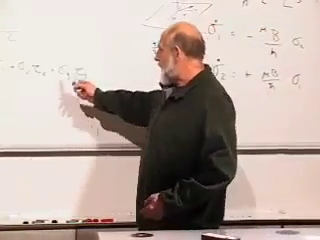
\includegraphics[width=0.75\textwidth]{lecture_09_figure_12.png}
\caption{各向同性双自旋相互作用\(H\propto\boldsymbol{\sigma}\cdot\boldsymbol{\tau}\)。}
\lectureframe{01:19:20}
\end{figure}

\begin{classroomqa}
\lecturetimestamp{01:17:49}
\audiencequestion{将两个纠缠电子置于均匀磁场中是否必然使它们退纠缠？}
\lecturerresponse{不一定。磁场改变哈密顿量，并可能倾向于使自旋对齐，尤其是在磁场很强时，但均匀磁场中的幺正演化本身并不保证纠缠的丧失。答案取决于完整的哈密顿量和初始态。}
\end{classroomqa}

\subsection{三重态与单态能量}

双自旋希尔伯特空间的维数为四。相互作用在三重态--单态基下是对角的：
\begin{align}
\ket{T_+}&=\ket{\uparrow\uparrow}, \\
\ket{T_0}&=
\frac{\ket{\uparrow\downarrow}+\ket{\downarrow\uparrow}}{\sqrt2}, \\
\ket{T_-}&=\ket{\downarrow\downarrow}, \\
\ket{S}&=
\frac{\ket{\uparrow\downarrow}-\ket{\downarrow\uparrow}}{\sqrt2}.
\end{align}
三个三重态共享一个能量\(E_T\)；单态具有另一个能量\(E_S\)。因此有四个独立的本征矢，但只有两个不同的能级。三重态能级是三度简并的。

\begin{figure}[htbp]
\centering
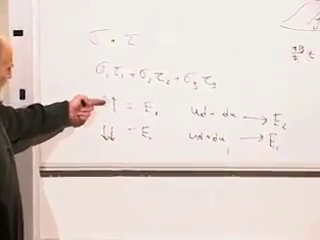
\includegraphics[width=0.74\textwidth]{lecture_09_figure_13.png}
\caption{耦合自旋哈密顿量具有一个简并的三重态能级和一个独立的单态能级。}
\lectureframe{01:20:30}
\end{figure}

\begin{classroomqa}
\lecturetimestamp{01:21:16}
\audiencequestion{如果初始态已经是单态能量本征态，会发生什么？}
\lecturerresponse{它保持为单态，只获得相位\(e^{-iE_St/\hbar}\)。与任何单一能量本征态一样，仅仅因为整个右矢乘以该共同相位，其可测量性质不会改变。}
\end{classroomqa}

\begin{classroomqa}
\lecturetimestamp{01:21:54}
\audiencequestion{在此计算过程中，外部磁场是否向双自旋系统提供能量？}
\lecturerresponse{所求解的示例中没有外部磁场。所讨论的唯一场是由\(J\,\boldsymbol{\sigma}\cdot\boldsymbol{\tau}\)表示的相互作用。添加外部磁场会给\(H\)增加另一项，并定义不同的问题。}
\end{classroomqa}

\subsection{从一个自旋向上和一个自旋向下开始}

能量本征态只会积累一个相位，因此选择一个不是能量本征态的乘积态：
\begin{equation}
\ket{\psi(0)}=\ket{\uparrow\downarrow}.
\end{equation}
将其分解为两个相关的本征矢：
\begin{equation}
\boxed{
\ket{\uparrow\downarrow}
=
\frac{1}{\sqrt2}\ket{T_0}
+
\frac{1}{\sqrt2}\ket{S}
}.
\end{equation}

\begin{figure}[htbp]
\centering
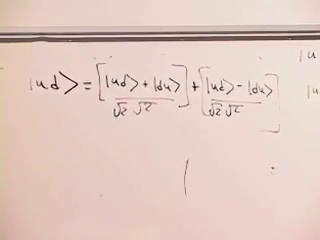
\includegraphics[width=0.76\textwidth]{lecture_09_figure_14.png}
\caption{乘积态 \(\ket{\uparrow\downarrow}\) 分解为三重态和单重态分量。}
\lectureframe{01:24:30}
\end{figure}

每个能量分量现在各自获得自己的相位：
\begin{equation}
\ket{\psi(t)}
=
\frac{e^{-iE_Tt/\hbar}}{\sqrt2}\ket{T_0}
+
\frac{e^{-iE_St/\hbar}}{\sqrt2}\ket{S}.
\end{equation}

\begin{classroomqa}
\lecturetimestamp{01:25:59}
\audiencequestion{三重态能量 \(E_T\) 和单重态能量 \(E_S\)，哪个更大？}
\lecturerresponse{这取决于耦合的符号。对于 \(H=J\,\boldsymbol{\sigma}\cdot\boldsymbol{\tau}\) 且 \(J>0\)，单重态更低而三重态更高；改变符号则颠倒次序。给两个能量同时加上一个常数只会改变一个整体相位，因此可以在不改变跃迁概率的前提下把任一能级设为零。}
\end{classroomqa}

回到乘积基：
\begin{align}
\ket{\psi(t)}
&=
\frac12
\left(
e^{-iE_Tt/\hbar}+e^{-iE_St/\hbar}
\right)\ket{\uparrow\downarrow} \\
&\quad+
\frac12
\left(
e^{-iE_Tt/\hbar}-e^{-iE_St/\hbar}
\right)\ket{\downarrow\uparrow}.
\end{align}

\begin{figure}[htbp]
\centering
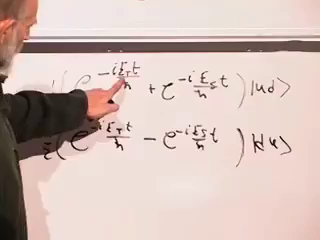
\includegraphics[width=0.76\textwidth]{lecture_09_figure_15.png}
\caption{演化后的态在 \(\ket{\uparrow\downarrow}\)、\(\ket{\downarrow\uparrow}\) 基中重新组合。}
\lectureframe{01:30:40}
\end{figure}

在 \(t=0\) 时，\(\ket{\downarrow\uparrow}\) 的系数为零，这是必然的。在之后的时刻，单重态与三重态分量之间的相对相位使该系数增大。定义平均能量与能级分裂，
\begin{equation}
\overline E=\frac{E_T+E_S}{2},
\qquad
\Delta E=E_T-E_S.
\end{equation}
提出平均能量的相位因子后得到
\begin{equation}
\boxed{
\begin{aligned}
\ket{\psi(t)}
&=e^{-i\overline E t/\hbar}\Biggl[
\cos\!\left(\frac{\Delta E\,t}{2\hbar}\right)
\ket{\uparrow\downarrow}
\\
&\qquad
-i\sin\!\left(\frac{\Delta E\,t}{2\hbar}\right)
\ket{\downarrow\uparrow}
\Biggr]
\end{aligned}
}.
\end{equation}

\begin{figure}[H]
\centering
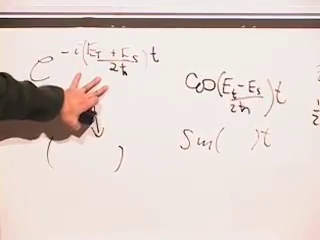
\includegraphics[width=0.76\textwidth]{lecture_09_figure_16.png}
\caption{平均能量成为一个公共相位，而单重态--三重态分裂则出现在正弦和余弦振幅中。}
\lectureframe{01:35:15}
\end{figure}

因子 \(e^{-i\overline E t/\hbar}\) 对整个右矢是公共的，会从每个概率中消去。可测量的概率为
\begin{equation}
P_{\uparrow\downarrow}(t)
=
\cos^2\!\left(\frac{\Delta E\,t}{2\hbar}\right),
\qquad
P_{\downarrow\uparrow}(t)
=
\sin^2\!\left(\frac{\Delta E\,t}{2\hbar}\right).
\end{equation}
该态在 \(\ket{\uparrow\downarrow}\) 与 \(\ket{\downarrow\uparrow}\) 之间来回振荡，其速率仅由能量差决定。在中间时刻两个振幅都非零，除特殊瞬间外两个自旋是纠缠的。

这一计算说明了一个普遍方法。选择物理问题所依据的基，将初态按哈密顿量的本征矢展开，让每个本征矢获得自己的相位，然后在测量基中把各部分重新组合。一旦哈密顿量被对角化，量子动力学就变得系统化；所有可观测的运动都由相对相位承载。
